\documentclass[12pt]{article}
\usepackage[utf8]{inputenc}
\usepackage[russian]{babel}
\usepackage{titlesec}
\usepackage{titling}
\usepackage{textcomp}
\usepackage{graphicx}
\usepackage{amssymb}
\usepackage[russian]{babel}
\usepackage[babel = true]{microtype}
\usepackage[left=10mm,right=10mm, top=15mm,bottom=15mm]{geometry}
\usepackage{amsmath}
\usepackage{mathtools}
\usepackage{array}
\usepackage{wrapfig}
\usepackage{multirow}
\usepackage{gensymb}
\usepackage{tabu}
\usepackage{graphicx}
\usepackage{subcaption}
\let\oldAA\AA
\renewcommand{\AA}{\text{\normalfont\oldAA}}

\makeatletter
\newcommand*{\rom}[1]{\expandafter\@slowromancap\romannumeral #1@}
\makeatother

\setlength{\droptitle}{-5em}

\title{4.5.1 Гелий-неоновый лазер}
\date{}

\titleformat{\section}[hang]
{\normalfont\bfseries}
{\thesection.}{0.5em}{}

\titleformat{\subsection}[hang]
{\normalfont\bfseries}
{\thesection.}{0.5em}{}

\begin{document}

\maketitle

\paragraph{Цель работы:}Изучение основных принципов работы гелий-неонового лазера, свойств лазерного излучения и измерение усиления лазерной трубки.

\paragraph{В работе используются:}объект исследования — активный элемент от гелий-неонового лазера ЛГ-75 с блоком питания, дополнительный He–Ne-лазер для юстировки и измерений, модулятор излучения (обтюратор), фотодиоды, зеркала, поляроид, компьютер со звуковой картой.

\section*{Теоретическая часть:}
\begin{enumerate}
    \item Гониометр служит для точного измерения углов.  
    
    \item Показатель преломления призмы. \\
    \begin{figure}[h!]
        \noindent\centering{
            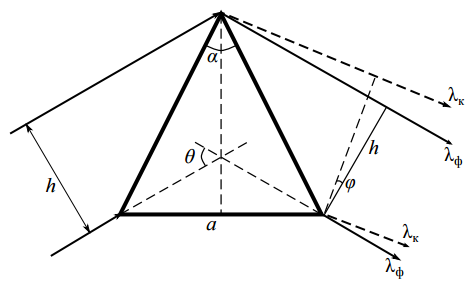
\includegraphics[height = 4cm]{1.png}
        }
        \caption{Призма.}
    \end{figure} \\
%    \newpage
    Минимальное отклонение луча, преломленного призмой, от направления луча, падающего на призму, получается при симметричном ходе луча
    ($\delta$ --- угол минимального отклонения, $\alpha$ --- преломляющий угол, $n$ --- показатель преломления): \\
    \begin{align}
        n = \frac{\sin{\frac{\alpha + \delta}{2}}}{\sin{\frac{\alpha}{2}}}
    \end{align} 
    
    \item Дисперсионная кривая --- график зависимости $n(\lambda)$ \\
        \begin{enumerate}
            \item средняя дисперсия: $D = n_F - n_C$
            \item коэффициент диспрсии: $\nu = \frac{n_D - 1}{n_F - n_C}$, где:
        \end{enumerate}
    $n_D$ --- показатель преломления для $\lambda_D = 589,3nm$ (среднее значения длин волн желтого дуплета натрия) \\
    $n_F$ --- показатель преломления для $\lambda_F = 486,1nm$ (голубая линия водорода) \\
    $n_C$ --- показатель преломления для $\lambda_C = 656,3nm$ (красная линия водорода) \\
    
    \item Разрешающая способность призмы: $R = \frac{\lambda}{\delta\lambda} = b \frac{dn}{d\lambda}$ \\
    $\delta\lambda$ --- минимальный интервал длин волн, разрешаемый по критерию Релея \\
    $b$ --- размер основания призмы, если вся рабочая грань призмы освещена параллельным пучком 
    
    \item Принцип Гюйгенса-Френеля:
    каждый элемент волнового фронта можно рассматривать как центр вторичных возмущений,
    порождающего вторичные сферические волны, а результирующее световое поле в каждой точке пространства
    будет определяться интерференцией этих волн. \\
    Дисперсия --- явления, обусловленные зависимостью абсолютного показателя преломления вещества от частоты света.
%    \item Получение эллиптически поляризованного света. \\
%    \begin{figure}[h!]
%        \noindent\centering{
%            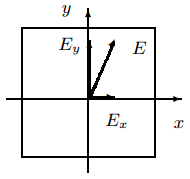
\includegraphics[height = 4cm]{Selection_048.png}
%        }
%        \caption{Разложение линейно поляризованного света по главным направлениям двоякопреломляющей пластинки.}
%    \end{figure} \\
    
\end{enumerate}
%\newpage
\section*{Экспериментальная установка:}
\begin{enumerate}
    \item Оптическая схема и внешний вид гониометра
    \begin{figure}[h!]
        \noindent\centering{
            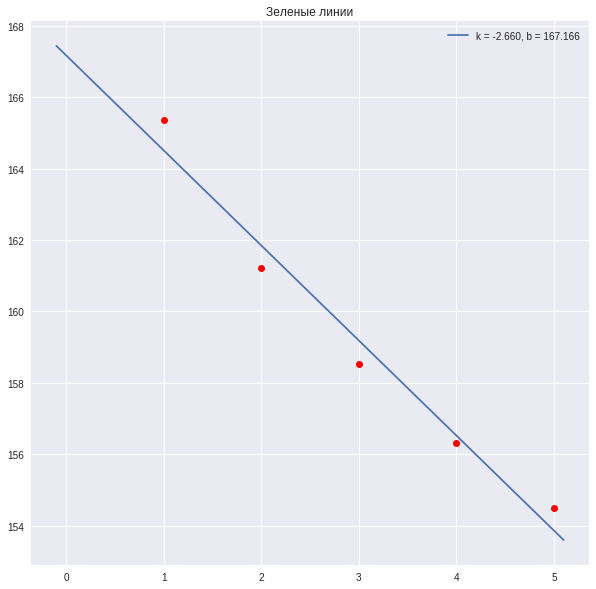
\includegraphics[height = 4cm]{2.png}
        }
    \end{figure} 
    
\end{enumerate}
\section*{Ход работы:}
\begin{enumerate}
    \item Определим разрешённые направления поляроидов.
    \begin{align*}
        \varphi_1 = 20 \\
        \varphi_2 = 160
    \end{align*}
    
    \item Определим угол Брюстера для эбонита \\
    Минимум интенсивности достигается при $\alpha = 58\degree$. Тогда имеем:
    $\tg{\alpha} = \frac{n_2}{n_1} = n$ \\
    $n = 1.6$
    
    \item Исследуем поляризацию света в преломленных и отраженных от стопы лучах. \\
    Установим стопу в таком положении, при котором свет падает на нее под углом Брюстера. \\
    Осветим стопу неполяризационным светом и рассмотрим через поляроиды. \\
    Видим, что в отраженном луче свет поляризован вертикально.
    
    \item Определим главных направлений стопы. \\
    Поставим пластину и поляроиды $P_1$ и $P_2$. Вращая пластины 1 и 2, находим минимумы интенсивности: \\
    $\alpha_1 = 112\degree,\ \alpha_2 = 110\degree$
    
    \item Выделение пластин $\lambda / 2$ и $\lambda / 4$. \\
    Установим разрешённое направление поляроида горизонтально, а главные направления исследуемой пластинки 
    — под углом $45\degree$ к горизонтали. С помощью второго поляроида определим, какую поляризацию имеет свет, прошедший пластинку. \\
    Пластинка 1 --- линейная, с переходом в квадрат --- $\lambda / 2$; \\
    Пластинка 2 --- круговая --- $\lambda / 4$.
    
    \item Определим направлений большей и меньшей скорости в пластинке $\lambda / 4$. \\
    Пластинка чувствительного оттенка не меняет поляризации зеленого света в условиях предыдущего опыта. \\
    При повороте рейтера оранжевый цвет переходиит в голубой. \\
    "Быстрая" ось соответствует голубому цвету.
    
    \item Интерференция поляризованных лучей. \\
    Пр вращении пластины наблюдаем, что при сохранении цвета меняется интенсивность. \\
    При вращении второго поляроида --- наоборот, меняется цвет.
    
\end{enumerate}
%\section*{Обработка результатов:}
\begin{enumerate}
    \item 
    \begin{align*}
        &R = \frac{\lambda}{\delta\lambda} = b \frac{dn}{d\lambda} \\
        &D = \frac{m}{\sqrt{d^2 - m^2 \lambda^2}} \\
        &m \cdot N = R \\
        &N = d \cdot n, \\
    \end{align*}
    где $m$ --- максимумы, $d = 1/n, n = 100$ штр/мм, $d$ --- длинна решетки. 
    
    \item Для каждой длинны волны определим показатель преломления: \\
    \begin{tabu} to 1\textwidth{|c|c|c|c|c|}
    \hline
    \lambda, nm & 404,7 & 491,6 & 546,1 & 578 \\
    \hline
    \delta  & 63\degree32'52" & 65\degree21'52" & 64\degree46'54" & 63\degree56'54" \\
    \hline
    $n$     & 1,7179    & 1,7315    & 1,7272    & 1,7209 \\
    \hline
    \end{tabu}
    
    \item Соответсвие длинн волн и показателя преломления: \\
    \begin{tabu}{|c|c|c|}
        \hline
        \lambda, nm & $n$ & \\
        \hline
        589,3 & 1,67 & d \\
        \hline
        486,1 & 1,72 & f \\
        \hline
        656,3 & 1,7 & c \\
        \hline
    \end{tabu}
    
    \item Найдем среднюю диспрсию и коэффициент диспрсии: \\
    $D = 0,02$ \\
    $\nu = 33,5$
    
    \item Найдем разрешающую способность призмы: \\
    $R = \frac{\lambda}{\delta\lambda} = 1964,33$ \\
    $b_\text{рабочая} = 0,039$ \\
    $R = b \frac{dn}{d\lambda} = 3500$

    \item И наконец, построим график зависимости $n(\lambda)$:
    \begin{figure}[h!]
        \noindent\centering{
            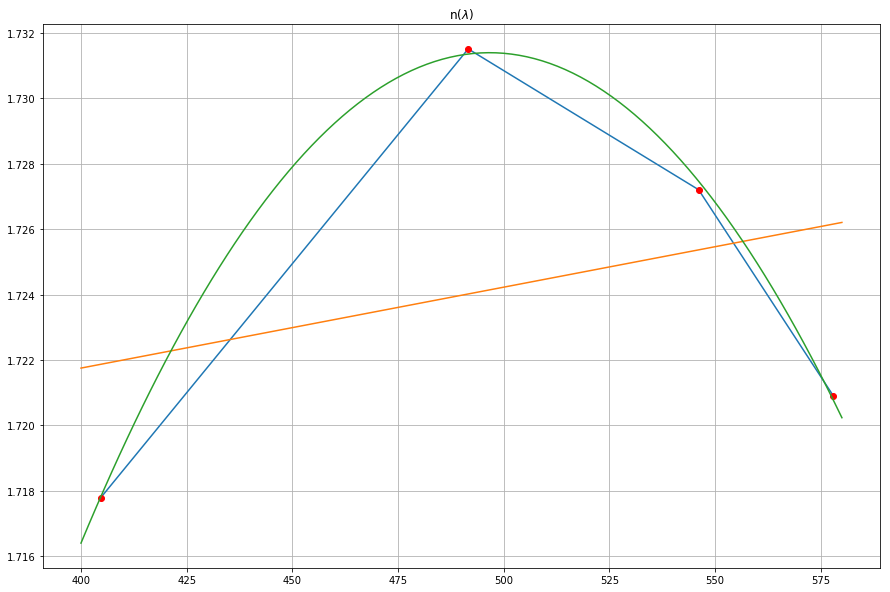
\includegraphics[height = 10cm]{3.png}
        }
    \end{figure} \\
    
\end{enumerate}

\section*{Вывод:} в данной работе мы ознакомились с принципами работы гелий-неонового лазера, установили его коэффициент усиления $k = 1,02 \pm 0,03$, убедлились в том, что генерируемое узлучение является поляризованным.

\end{document}